\chapter{Các mô hình mạng tham khảo chính}
% \section{Định hướng phát triển mô hình}
\section{Mạng đảo tích chập cơ bản dùng cho phân đoạn ảnh}
Trong bối cảnh các mô hình mạng học sâu tích chập (Convolution neural networks - CNN) đã cho thấy khả năng phân loại ảnh vượt bậc, nhiều mô hình mới dựa trên kiến trúc này để giải quyết bài toán khác dần được phát triển và có được kết quả rất khả quan. Trong đó có thể đến như \cite{object_detection_ex1} và \cite{object_detection_ex2} để nhận diện vị trí vật thể, \cite{segmentation_ex1} và \cite{segmentation_ex2} để phân đoạn vật thể, \cite{action_recognize_ex1} để nhận diện hành vi người.\\
Trong đó, các mạng dùng để phân đoạn ảnh dựa trên CNN sẽ được chuyển về mạng tích chập đầy đủ (Fully Convolutional Network) bằng cách loại bỏ tất cả các lớp liên kết đầy đủ và thay thế bằng cách lớp tích chập. Các mạng FCN này sẽ gán nhẵn cho từng điểm ảnh và thực hiện một phép phóng to ảnh cơ bản bằng phương pháp nội suy. Một số công trình giới thiệu kết quả tốt hơn bằng việc sử dụng trường điều kiện ngẫu nhiên sau khi đã sử dụng mạng học sâu.\\
Các phương án phân đoạn ảnh vừa nêu đều có một số hạn chế nhất định. Khi sử dụng giải pháp phóng lớn ảnh bằng phương pháp nội suy điểm ảnh, ảnh kết quả thường bị thô và nhoè vì với phương pháp này giá trị điểm ảnh mới có độ chính xác không cao. Còn khi sử dụng trường điều kiện ngẫu nhiên để làm mượt ảnh, tốc độ rất hạn chế và đòi hỏi máy tính phải có cấu hình mạnh, đặc biệt khi sử dụng phương pháp này cho một ảnh 3-chiều. Để giải quyết các hạn chế đó, Hyeonwoo Noh và cộng sự giới thiệu mô hình mạng đảo tích chập \cite{unpoolref} theo thiết kế của một mạng tích chập đầy đủ (FCN).
\subsection{Kiến trúc mạng}
Mạng đảo tích chập của Hyeonwoo và cộng sự sử dụng kiến trúc mã hoá và giải mã quen thuộc của các mạng phân đoạn. Mô hình mạng này là một cải tiến của loại mạng VGG16 với các điểm đặc biệt sau:
\begin{itemize}
    \item Phần mã hoá sử dụng các khối mạng gồm các lớp tích chập và gộp có số lượng và cấu hình như mạng VGG16. 
    \item Loại bỏ các lớp kết nối đầy đủ ở VGG16, thay bằng các lớp tích chập. Phần mã hoá trở thành một phiên bản FCN của VGG16.
    \item Phần giải mã thiết kế đối xứng với phần mã hoá.
    \item Kích thước ảnh ở đầu vào và đầu ra của mạng là giống nhau.
\end{itemize}
\begin{figure}[h]
\centering
    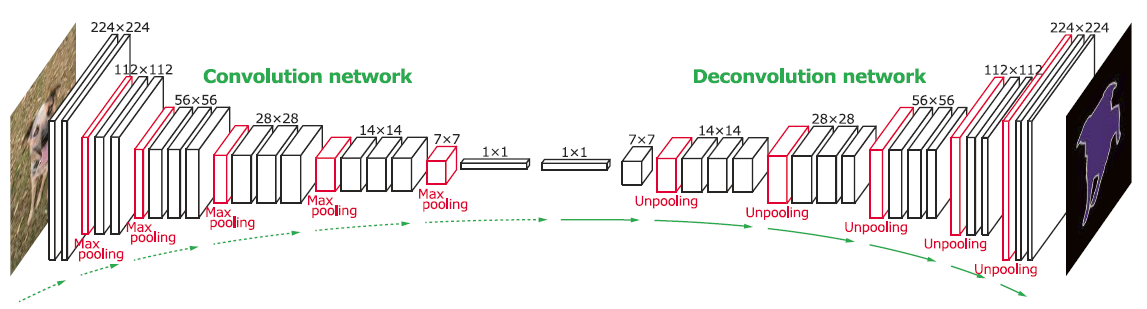
\includegraphics[totalheight=4cm]{Images/deconvNet.png}
    \caption{Mô hình mạng đảo tích chập của Hyeonwoo Noh và cộng sự}
    \label{deconvNet}
\end{figure}

\subsection{Các lớp mạng}
Trong \cite{unpoolref}, Hyeonwoo và cộng sự đã có một thay đổi nhỏ ở phần mã hoá so với VGG16 đó là sử dụng lớp chuẩn hoá (Batchnorm) để tránh tình trạng bão hoà gradient khiến mạng không thể được cập nhật trọng số. Các lớp chuẩn hoá này được thiết kế đặt sau mỗi lớp tích chập và lớp đảo tích chập. Theo các tác giả, lớp chuẩn hoá được thêm vào do chiều sâu của mạng đảo tích chập đã được tăng lên gấp đôi so với VGG16, thay đổi này nhằm tránh lại nhược điểm khó học của các mạng có độ sâu quá lớn.\\
Các lớp gộp được thiết kế để loại bớt giá trị nhiễu bằng cách sử dụng một giá trị đại diện cho một vùng ảnh. Mặc dù mang tính chất đại diện cho nhiều điểm ảnh, nhưng cách làm như vậy lại vô tình khiến mạng bị mất thông tin. Để giải quyết vấn đề này, mạng đảo tích chập sử dụng một bảng nhớ và dùng nó lại trong quá trình đảo gộp. Chi tiết xem tại mục phép đảo gộp trình bày ở chương Cơ sở lý thuyết.\\
Để xây dựng lại ảnh phân đoạn có kích thước ảnh gốc trong quá trình giải mã. Mạng đảo tích chập sử dụng phép đảo tích chập có kích thước và số các ma trận lõi gần như đối xứng với phần mã hoá. Tuy nhiên, số ma trận lõi của lớp tích chập ở trước mỗi lớp đảo gộp bị giảm đi một nửa so với các lớp tích chập khác trong khối mã hoá.\\
Tất cả các hàm kích hoạt được sử dụng là hàm Relu, trừ lớp đảo tích chập cuối cùng sử dụng hàm softmax để phù với mục đích phân đoạn của bài toán cho nhiều lớp đối tượng (class).
\subsection{Huấn luyện mạng}
Trong \cite{unpoolref}, mạng đảo tích chập được huấn luyện để sử dụng phân đoạn cho bộ dữ liệu PASCAL VOC 2012. Hyeonwoo và cộng sự sử dụng các trọng số trong phần mã hoá đã được huấn luyện cho mạng VGG16 với tập ILSVRC (pretrain). Quá trình huấn luyện sử dụng tốc độ học (learning rate) 0.01, đà (momentum) 0.9, khử trọng số (weight decay) 0.0005.

\section{Mô hình mạng đảo tích chập với phương pháp huấn luyện giám sát sâu (DSN)}
Trong bài toán phân đoạn ảnh, mạng nơ-ron tích chập với kiến trúc mã hóa, giải mã (encoder - decoder) là một trong những mô hình học sâu truyền thống được sử dụng rộng rãi nhất. Kỹ thuật huấn luyện mô hình này bằng phương pháp giám sát sâu đã được giới thiệu trong bài báo "3D Deeply Supervised Network for Automatic Liver Segmentation from CT Volumes" bởi Qi Dou và cộng sự\cite{dsn_paper}.
Khi huấn luyện mô hình (Train time), hai lớp giải mã tương ứng được thêm vào mạng tạo ra phần "Deep Supervision". Như vậy, mô hình lúc này sẽ có ba cổng ra và đồng thời cũng sẽ có ba hàm mất mát tương ứng với từng cổng ra. Hàm mất mát toàn phần lúc này là tổng hợp giữa hàm mất mát chính và các hàm mất mát phụ:\\
\begin{center} $Loss = \mu_1 Loss_{6} + \mu_2 Loss_{3} + \mu_3 Loss_{main}$\end{center}
\begin{figure}[h]
\centering
    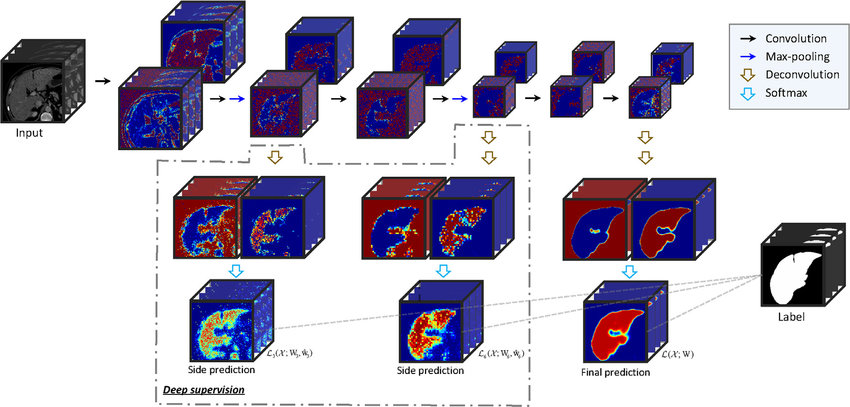
\includegraphics[totalheight=8cm]{Images/The-architecture-of-the-proposed-3D-DSN-taking-3D-liver-segmentation-as-an-example.png}
    \caption{Kiến trúc mô hình mạng đảo tích chập với phương pháp huấn luyện giám sát sâu (DSN)}
    \label{DSN}
\end{figure}
Với phương pháp huấn luyện mô hình này, trọng số trên phần mã hóa sẽ được cập nhật và chia sẽ giữa các luồng thay vì chỉ trên luồng chính. Việc này nhằm tăng khả năng học các đặc trưng quan trọng giúp phân đoạn chính xác lá gan, đồng thời giảm khả năng "vanishing gradient".
\section{Mô hình mạng Unet}
Mô hình mạng Unet được giới thiệu trong bài báo "U-Net: Convolutional Networks for Biomedical Image Segmentation" vào ngày 18 tháng 5 năm 2015 bởi Olaf và các cộng sự.\cite{unet_paper}\\
Mạng Unet là sự kết hợp của các lớp tích chập, lớp gộp, lớp gộp kênh và lớp phóng lớn kích thước mẫu (up-sampling). Tên mạng Unet được đặt theo kiến trúc giống hình chữ U của mạng với hai phần gần như đối xứng nhau. Mạng Unet có kiến trúc tương tự với các mạng sử dụng cho mục đích phân đoạn ảnh khác khi kiến trúc mạng có thể chia ra hai phần là mã hoá (encoder) và giải mã (decoder). Điểm khác biệt của mạng Unet là cách xử lý trong quá trình làm lơn kích thước mẫu khi sử dụng các kết nối tắt từ phần mã hoá đến phần giải mã. Qua đó kết quả phân đoạn được làm tốt hơn đáng kể. Phần sau đây sẽ trình bày lại các chi tiết hơn các đặc điểm mạng Unet của Olaf và các cộng sự. 
\subsection{Kiến trúc phần mã hoá}
Phần mã hoá của mạng sử dụng các lớp tích chập và lớp gộp như các mạng dùng cho xử lý ảnh khác. Tuy nhiên so với các mạng dùng cho xác định, phân loại ảnh như VGG16, VGG19, Resnet, thì Unet có độ sâu nhỏ hơn. Mạng Unet tô chức các lớp tích chập và gộp với nhau thành những khối mã hoá, mỗi khối gồm hai lớp tích chập và một lớp gộp sau cùng (trừ khối cuối cùng không có lớp gộp là là khối trung gian giữa giải mã và mã hoá). Tuỳ vào mục đích sử dụng và tình huống khác nhau, các siêu tham số của các lớp này sẽ được cấu hình khác nhau. Thông thường, các lớp này sử dụng các ma trận lõi có kích thước 3x3, số ma trận lõi mỗi lớp của khối sau sẽ gấp đôi khối trước, hàm kích hoạt là Relu, khối gộp sử dụng hàm lớn nhất với ma trận 2x2. Phần mã hoá này có tác dụng tìm ra các đặc điểm chung và phổ quát của ảnh đầu vào, chấp nhận mất mát thông tin trong quá trình.

\subsection{Kết nối tắt}
Ở mỗi khối mã hoá, trước khi ảnh được xử lý gộp sẽ có một kết nối để giữ những giá trị chưa gộp này và đưa chúng vào một khối giải mã. Kết nối đầy đủ này xuất hiện trước tất cả các lớp gộp. Như vậy, nhược điểm của các lớp gộp là làm mất thông tin giờ đã được khắc phục bằng các kết nối tắt, có tác dụng giữ lại tất cả các thông tin có thể mất mát do quá trình gộp để dùng cho quá trình giải mã, giúp cho ảnh phân đoạn cuối cùng trở nên chi tiết hơn.

\begin{figure}[h]
\centering
    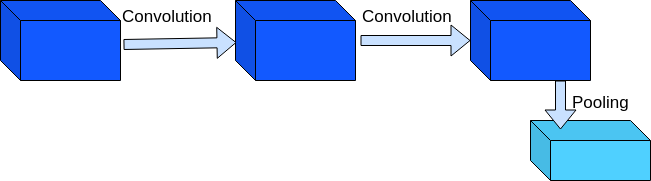
\includegraphics[totalheight=3cm]{Images/encoder_block.png}
    \caption{Dữ liệu được xử lý trong mỗi khối mã hoá}
    \label{skip_conn}
\end{figure}

\begin{figure}[h]
\centering
    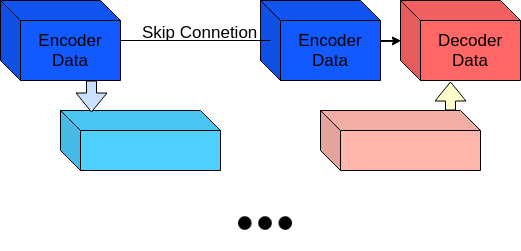
\includegraphics[totalheight=4.5cm]{Images/skip_conn.png}
    \caption{Dữ liệu truyền qua kết nối tắt}
    \label{skip_conn}
\end{figure}

\begin{figure}[h]
\centering
    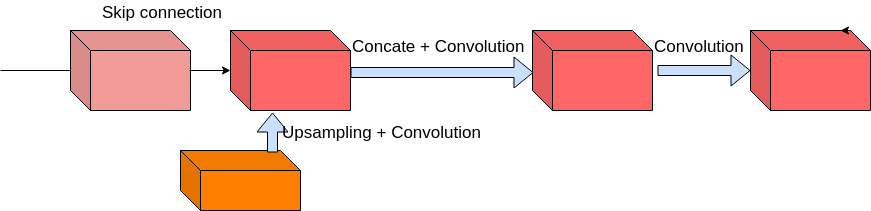
\includegraphics[totalheight=3.45cm]{Images/decoder_block.png}
    \caption{Dữ liệu được xử lý trong khối giải mã}
    \label{skip_conn}
\end{figure}

\subsection{Kiến trúc phần giải mã}
Phần mã hoá thông tin có tác dụng tìm ra những đặc điểm phổ quát của ảnh, còn phần giải mã có tác dụng tạo ra kết quả phân đoạn từ những thông tin đã được mã hoá. Phần giải mã được cấu tạo từ các lớp phóng lớn, lớp nối kênh và lớp tích chập thành các khối giải mã. Khối giải mã có cấu trúc gần đối xứng với khối mã hoá gồm lần lượt một khối tăng kích thước, một khối tích chập, một khối nối kênh, hai khối tích chập. Cấu hình siêu tham số các lớp giải mã giống với cấu hình siêu tham số các lớp ở quá trình mã hoá. Dữ liệu từ lớp trung gian khi đi qua từng khối giải mã sẽ được lớp phóng to làm lớn gấp đôi, các lớp tích chập sử dụng số ma trận lõi có kích thước 3x3, số ma trận lõi của lớp trước gấp đôi lớp sau, lớp cộng kênh được sử dụng cho kết quả lớp phóng lớn và dữ liệu của kết nối tắt.

\begin{figure}[h]
\centering
    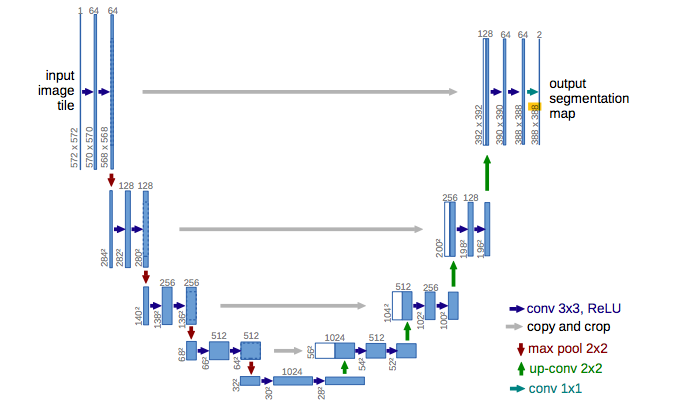
\includegraphics[totalheight=9.5cm]{Images/unet.png}
    \caption{Toàn bộ kiến trúc mạng Unet}
    \label{skip_conn}
\end{figure}

\subsection{Hàm lỗi}
Trong \cite{unet_paper}, Olaf và cộng sự sử dụng hàm lỗi cross-entropy. Tuy nhiên tuỳ vào đặc tính các tập dữ liệu khác nhau, mà nhiều hàm lỗi khác nhau có thể được sử dụng như hàm Dice, hàm cross-entropy với trọng số.

\subsection{Mạng Unet 3-chiều}
Trong \cite{3DUnet}, Ozgun Cikek và cộng sự đã giới thiệu một mô hình mạng Unet 3-chiều dùng cho xử lý các ảnh cắt lớp được tổ chức chung với nhau thành một khối và có thể coi như một ảnh 3-chiều, đây là định dạng của các ảnh CT và MRI.\\
So với mạng Unet, mạng Unet 3-chiều của Ozgun Cikek và cộng sự có một số điểm khác biệt sau:
\begin{itemize}
    \item Sử dụng ảnh đầu vào là các ảnh chụp lát cắt liên tục.
    \item Sử dụng các ma trận lõi 3-chiều, thực hiện phép tính tích chập, gộp, gộp kênh 3-chiều.
    \item Giảm số khối mã hoá và giải mã (từ 4 khối về 3 khối).
    \item Giảm số ma trận lõi ở mỗi lớp tích chập.
    \item Gấp đôi số kênh bằng cách gấp đôi số ma trận lõi trước khi thực hiện phép gộp (Unet của Olaf thực hiện sau) nhằm giảm thiểu sự mất mát dữ liệu.
    \item Sử dụng phép chuẩn hoá (batchnorm) sau các hàm kích hoạt.
\end{itemize}

\begin{figure}[h]
\centering
    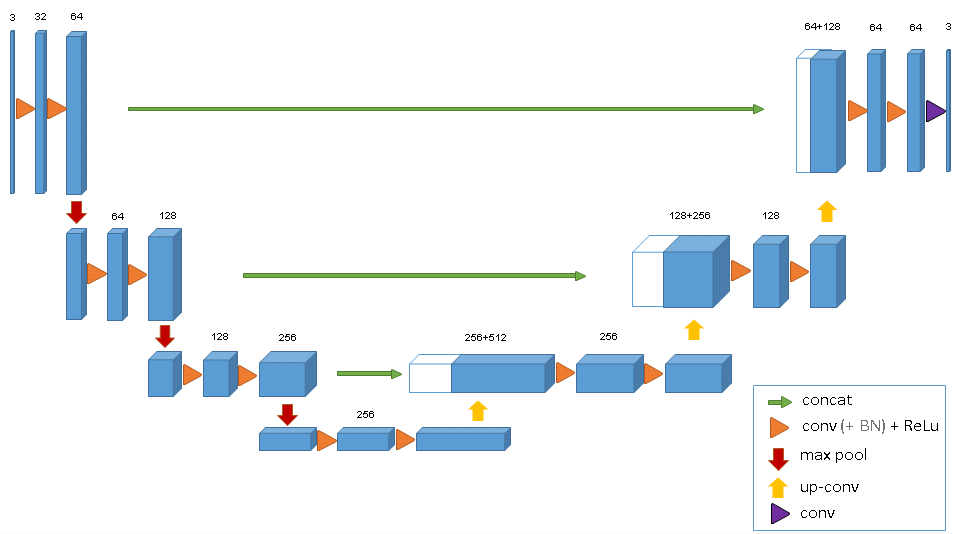
\includegraphics[totalheight=7cm]{Images/3Dunet.png}
    \caption{Kiến trúc mạng Unet 3-chiều}
    \label{skip_conn}
\end{figure}



